\documentclass[submit]{harvardml}
% \documentclass[submit]
% \course{CS1810-S25}
\assignment{Homework \#4}
\duedate{April 3, 2026 at 11:59pm}

\usepackage[OT1]{fontenc}
\usepackage[colorlinks,citecolor=blue,urlcolor=blue]{hyperref}
\usepackage[pdftex]{graphicx}
\usepackage{caption}
\usepackage{fullpage}
\usepackage{soul}
\usepackage{amsmath}
\usepackage{amssymb}
\usepackage{framed}
\usepackage{color}
\usepackage{todonotes}
\usepackage{listings}
\usepackage{common}
\usepackage{float,booktabs}
\newcommand{\E}{\mathbb{E}}
\newcommand{\KL}{D_{\mathrm{KL}}}
\newcommand{\R}{\mathbb{R}}
\newcommand{\bx}{\mathbf{x}}
\newcommand{\bz}{\mathbf{z}}

%%%%%%%%%%%%%%%%%%%%%%%%%%%%%%%%%%%%%%%%%%%
%% Solution environment
\usepackage{xcolor}
\newenvironment{solution}{
    \vspace{2mm}
    \color{blue}\noindent\textbf{Solution}:
}{}
%%%%%%%%%%%%%%%%%%%%%%%%%%%%%%%%%%%%%%%%%%%

\usepackage[mmddyyyy,hhmmss]{datetime}

\definecolor{verbgray}{gray}{0.9}

\lstnewenvironment{csv}{
  \lstset{backgroundcolor=\color{verbgray},
  frame=single,
  framerule=0pt,
  basicstyle=\ttfamily,
  columns=fullflexible}}{}
 
\begin{document}

\begin{center}
{\Large Representation Learning, Transformers, and Non-parametric methods}\\
\end{center}

\subsection*{Introduction}

This homework contains three problems:
\begin{enumerate}
    \item You will do some transformer computations by hand, and implement self-attention from scratch and produce attention score heatmaps.
    \item You will do some derivations related to autoencoders and implement them.
    \item You will do some math to prove bounds on decision tree ensembles, in order to 
\end{enumerate}

We note that this homework does not have any problem where you directly run through the computations you would do to derive a decision tree. Doing so can be good review, however, so for an example with those computations, please see the last exercise in Section 6 notes.

\subsection*{Resources and Submission Instructions}

Please type your solutions after the corresponding problems using this \LaTeX\ template, and start each main problem on a new page.

Please submit the writeup PDF to the Gradescope assignment `HW4'. Remember to assign pages for each question.  \textbf{You must include any plots in your writeup PDF. }. Please submit your \LaTeX file and code files to the Gradescope assignment `HW4 - Supplemental.' The supplemental files will only be checked in special cases, e.g. honor code issues, etc. Your files should be named in the same way as we provide them in the repository, e.g. \texttt{hw4.pdf}, etc.




\newpage

%%%%%%%%%%%%%%%%%%%%%%%%%%%%%%%%%%%%%%%%%%%%%
% Problem : Understanding the Transformer
%%%%%%%%%%%%%%%%%%%%%%%%%%%%%%%%%%%%%%%%%%%%%

\begin{problem}[Understanding the Transformer, 40 pts]

Transformers are the dominant architecture behind large language models and many modern
sequence processing systems.  At the heart of every transformer is \textbf{self-attention},
a mechanism that allows each position in a sequence to ``look at'' every other position
and decide how much information to gather from each.

In this problem you will (a)~work through the math of scaled dot-product attention,
(b)~understand key design choices, and (c)~implement the attention layer.

\medskip\noindent
\textbf{Background.}
Given an input matrix $\boldX \in \reals^{T \times d}$ (one row per token),
self-attention computes:
\[
  \text{Attention}(\boldQ, \boldK, \boldV)
  = \text{softmax}\!\left(\frac{\boldQ \boldK^\trans}{\sqrt{d_k}}\right)\boldV,
\]
where $\boldQ = \boldX \boldW_Q$, $\boldK = \boldX \boldW_K$,
$\boldV = \boldX \boldW_V$ with learnable weight matrices
$\boldW_Q, \boldW_K \in \reals^{d \times d_k}$ and
$\boldW_V \in \reals^{d \times d_v}$.
The softmax is applied row-wise: for a row vector $\boldz \in \reals^T$,
$\text{softmax}(\boldz)_i = e^{z_i} / \sum_{j=1}^{T} e^{z_j}$.

\begin{enumerate}

%%% Part (a) %%%
\item \textbf{[10 pts] Attention by hand.}

Consider a sequence of $T = 2$ tokens with embedding dimension $d = 2$. The input
matrix, query weight matrix, key weight matrix, and value weight matrix are:
\[
  \boldX = \begin{pmatrix} 1 & 0 \\ 0 & 1 \end{pmatrix}, \quad
  \boldW_Q = \begin{pmatrix} 1 & 1 \\ 0 & 1 \end{pmatrix}, \quad
  \boldW_K = \begin{pmatrix} 1 & 0 \\ 1 & 1 \end{pmatrix}, \quad
  \boldW_V = \begin{pmatrix} 2 & 0 \\ 0 & 1 \end{pmatrix}.
\]
So $d_k = d_v = 2$.

\begin{enumerate}
  \item Compute $\boldQ$, $\boldK$, $\boldV$, and the raw score matrix
  $\boldS = \boldQ \boldK^\trans$.

  \item Compute the scaled score matrix $\boldS / \sqrt{d_k}$.
  Then apply softmax row-wise to obtain the attention weight matrix
  $\boldA \in \reals^{2 \times 2}$.

  You may leave your answer in terms of $e^{(\cdot)}$ and sums, or compute
  decimal approximations.
\end{enumerate}
%%% Part (b) %%%
\item \textbf{[5 pts] Why scale by $\sqrt{d_k}$\,?}

Suppose the entries of $\boldq, \boldk \in \reals^{d_k}$ are independent random
variables with mean~$0$ and variance~$1$.

\begin{enumerate}
  \item Compute the mean and variance of the dot product
  $\boldq^\trans \boldk = \sum_{i=1}^{d_k} q_i k_i$.

  \item As $d_k$ grows, what happens to the magnitude of $\boldq^\trans \boldk$?
  Explain in one or two sentences what effect this has on the softmax distribution
  (i.e.\ does it become more uniform or more peaked?).

  \item Show that after scaling by $1/\sqrt{d_k}$ the dot product has variance~$1$
  regardless of $d_k$.
\end{enumerate}

%%% Part (c) %%%
\item \textbf{[5 pts] Permutation equivariance.}

Let $\boldP_\sigma \in \reals^{T \times T}$ be the permutation matrix corresponding
to a permutation $\sigma$ of $\{1, \dots, T\}$ (i.e.\ $(\boldP_\sigma)_{ij} =
\mathbf{1}[j = \sigma(i)]$).

\begin{enumerate}
  \item Show that self-attention (without positional encoding) is
  \textbf{permutation equivariant}: if we permute the input rows by replacing
  $\boldX$ with $\boldP_\sigma \boldX$, the output is permuted in the same way.
  That is, show
  \[
    \text{Attention}(\boldP_\sigma \boldX) = \boldP_\sigma \, \text{Attention}(\boldX).
  \]
  \textit{Hint}: What happens to $\boldQ$, $\boldK$, $\boldV$, and the softmax
  when you left-multiply $\boldX$ by $\boldP_\sigma$?

  \item Explain in two or three sentences why permutation equivariance is a
  problem for tasks like language modeling, where word order matters.

  \item The standard fix is to add a \textbf{positional encoding}
  $\boldP\boldE \in \reals^{T \times d}$ to the input:
  $\boldX' = \boldX + \boldP\boldE$.
  Why does this break permutation equivariance?
\end{enumerate}

%%% Part (d) %%%
\item \textbf{[10 pts] Implementing self-attention from scratch (code).}

In the accompanying notebook, implement single-head scaled dot-product self-attention
using \textbf{only NumPy} (do not use pre-existing implementations such as PyTorch and sklearn).

Your function should take:
\begin{itemize}
  \item $\boldX \in \reals^{T \times d}$: input embeddings
  \item $\boldW_Q \in \reals^{d \times d_k}$, $\boldW_K \in \reals^{d \times d_k}$,
        $\boldW_V \in \reals^{d \times d_v}$: weight matrices
\end{itemize}
and return:
\begin{itemize}
  \item $\text{output} \in \reals^{T \times d_v}$: the attention output
  \item $\text{weights} \in \reals^{T \times T}$: the attention weight matrix $\boldA$
\end{itemize}

\textbf{Implementation tips}:
\begin{itemize}
  \item For numerical stability, before applying softmax to a row~$\boldz$, subtract
  $\max(\boldz)$: compute $\text{softmax}(\boldz - \max(\boldz))$. (As an aside, note that this does not change the softmax function.)
  % \item Test your implementation against the provided test cases.
\end{itemize}

%%% Part (e) %%%
\item \textbf{[10 pts] Multi-head attention}

In the notebook, extend your implementation to \textbf{multi-head attention}
and use it inside a small transformer classifier trained on a synthetic
sequence dataset.

Given $h$ heads, each head
  uses its own $\boldW_Q^{(i)}, \boldW_K^{(i)} \in \reals^{d \times d_k}$ and
  $\boldW_V^{(i)} \in \reals^{d \times d_v}$, where $d_k = d_v = d / h$.
  The outputs of all heads are concatenated and projected:
  \[
    \text{MultiHead}(\boldX) = [\text{head}_1 \,;\, \cdots \,;\, \text{head}_h]\,
    \boldW_O,
  \]
  where $\boldW_O \in \reals^{d \times d}$.

After training, attach one learned attention matrix as a heatmap and
briefly describe what it suggests the model is attending to.


\end{enumerate}

\end{problem}


\newpage


\begin{solution}
	\begin{enumerate}
	    \item \begin{enumerate}
	        \item \[
X=\begin{pmatrix}
1 & 0\\
0 & 1
\end{pmatrix},
\qquad
W_Q=\begin{pmatrix}
1 & 1\\
0 & 1
\end{pmatrix},
\qquad
W_K=\begin{pmatrix}
1 & 0\\
1 & 1
\end{pmatrix},
\qquad
W_V=\begin{pmatrix}
2 & 0\\
0 & 1
\end{pmatrix}.
\]

Since \(X = I_2\), we immediately get
\[
Q = XW_Q = W_Q = \begin{pmatrix}
1 & 1\\
0 & 1
\end{pmatrix},
\]
\[
K = XW_K = W_K = \begin{pmatrix}
1 & 0\\
1 & 1
\end{pmatrix},
\]
\[
V = XW_V = W_V = \begin{pmatrix}
2 & 0\\
0 & 1
\end{pmatrix}.
\]

Now compute the raw score matrix
\[
S = QK^\top.
\]

First,
\[
K^\top = \begin{pmatrix}
1 & 1\\
0 & 1
\end{pmatrix}.
\]

Therefore,
\[
S
=
\begin{pmatrix}
1 & 1\\
0 & 1
\end{pmatrix}
\begin{pmatrix}
1 & 1\\
0 & 1
\end{pmatrix}
=
\begin{pmatrix}
1\cdot 1 + 1\cdot 0 & 1\cdot 1 + 1\cdot 1\\
0\cdot 1 + 1\cdot 0 & 0\cdot 1 + 1\cdot 1
\end{pmatrix}
=
\begin{pmatrix}
1 & 2\\
0 & 1
\end{pmatrix}.
\]

Hence,
\[
Q=\begin{pmatrix}
1 & 1\\
0 & 1
\end{pmatrix},
\qquad
K=\begin{pmatrix}
1 & 0\\
1 & 1
\end{pmatrix},
\qquad
V=\begin{pmatrix}
2 & 0\\
0 & 1
\end{pmatrix},
\qquad
S=\begin{pmatrix}
1 & 2\\
0 & 1
\end{pmatrix}.
\]
\item Since \(d_k = 2\), we have \(\sqrt{d_k} = \sqrt{2}\). From part (a),
\[
S=\begin{pmatrix}
1 & 2\\
0 & 1
\end{pmatrix}.
\]

Therefore, the scaled score matrix is
\[
\frac{S}{\sqrt{d_k}}
=
\frac{1}{\sqrt{2}}
\begin{pmatrix}
1 & 2\\
0 & 1
\end{pmatrix}
=
\begin{pmatrix}
\frac{1}{\sqrt{2}} & \frac{2}{\sqrt{2}}\\[4pt]
0 & \frac{1}{\sqrt{2}}
\end{pmatrix}
=
\begin{pmatrix}
\frac{1}{\sqrt{2}} & \sqrt{2}\\[4pt]
0 & \frac{1}{\sqrt{2}}
\end{pmatrix}.
\]

Now apply softmax row-wise.

For the first row,
\[
\operatorname{softmax}\!\left(\frac{1}{\sqrt{2}}, \sqrt{2}\right)
=
\left(
\frac{e^{1/\sqrt{2}}}{e^{1/\sqrt{2}}+e^{\sqrt{2}}},
\frac{e^{\sqrt{2}}}{e^{1/\sqrt{2}}+e^{\sqrt{2}}}
\right).
\]

For the second row,
\[
\operatorname{softmax}\!\left(0,\frac{1}{\sqrt{2}}\right)
=
\left(
\frac{1}{1+e^{1/\sqrt{2}}},
\frac{e^{1/\sqrt{2}}}{1+e^{1/\sqrt{2}}}
\right).
\]

Hence the attention weight matrix is
\[
A=
\begin{pmatrix}
\frac{e^{1/\sqrt{2}}}{e^{1/\sqrt{2}}+e^{\sqrt{2}}}
&
\frac{e^{\sqrt{2}}}{e^{1/\sqrt{2}}+e^{\sqrt{2}}}
\\[10pt]
\frac{1}{1+e^{1/\sqrt{2}}}
&
\frac{e^{1/\sqrt{2}}}{1+e^{1/\sqrt{2}}}
\end{pmatrix}.
\]

Using decimal approximations,
\[
\frac{1}{\sqrt{2}} \approx 0.7071,\qquad \sqrt{2}\approx 1.4142,
\]
so
\[
A \approx
\begin{pmatrix}
0.3302 & 0.6698\\
0.3302 & 0.6698
\end{pmatrix}.
\]
	    \end{enumerate}
        \item \begin{enumerate}
            \item Let
\[
q = (q_1,\dots,q_{d_k})^\top, \qquad k = (k_1,\dots,k_{d_k})^\top,
\]
where the entries \(q_i\) and \(k_i\) are independent random variables with
\[
\mathbb{E}[q_i]=0,\quad \mathbb{E}[k_i]=0,\quad \operatorname{Var}(q_i)=1,\quad \operatorname{Var}(k_i)=1.
\]

We want the mean and variance of
\[
q^\top k = \sum_{i=1}^{d_k} q_i k_i.
\]

First, compute the mean:
\[
\mathbb{E}[q^\top k]
=
\mathbb{E}\!\left[\sum_{i=1}^{d_k} q_i k_i\right]
=
\sum_{i=1}^{d_k} \mathbb{E}[q_i k_i].
\]
Since \(q_i\) and \(k_i\) are independent,
\[
\mathbb{E}[q_i k_i] = \mathbb{E}[q_i]\mathbb{E}[k_i] = 0\cdot 0 = 0.
\]
Therefore,
\[
\mathbb{E}[q^\top k] = 0.
\]

Now compute the variance:
\[
\operatorname{Var}(q^\top k)
=
\operatorname{Var}\!\left(\sum_{i=1}^{d_k} q_i k_i\right).
\]
Because the pairs \((q_i,k_i)\) are independent across \(i\), the random variables \(q_i k_i\) are independent across \(i\), so
\[
\operatorname{Var}(q^\top k)
=
\sum_{i=1}^{d_k} \operatorname{Var}(q_i k_i).
\]

For each \(i\),
\[
\operatorname{Var}(q_i k_i)
=
\mathbb{E}[q_i^2 k_i^2] - \bigl(\mathbb{E}[q_i k_i]\bigr)^2.
\]
Since \(\mathbb{E}[q_i k_i]=0\),
\[
\operatorname{Var}(q_i k_i)=\mathbb{E}[q_i^2 k_i^2].
\]
Using independence again,
\[
\mathbb{E}[q_i^2 k_i^2] = \mathbb{E}[q_i^2]\mathbb{E}[k_i^2].
\]
Now
\[
\mathbb{E}[q_i^2] = \operatorname{Var}(q_i) + (\mathbb{E}[q_i])^2 = 1+0=1,
\]
and similarly
\[
\mathbb{E}[k_i^2]=1.
\]
Hence
\[
\operatorname{Var}(q_i k_i)=1\cdot 1=1.
\]
So
\[
\operatorname{Var}(q^\top k)=\sum_{i=1}^{d_k} 1 = d_k.
\]

Thus,
\[
\boxed{\mathbb{E}[q^\top k]=0,\qquad \operatorname{Var}(q^\top k)=d_k.}
\]
\item As \(d_k\) grows, the dot product \(q^\top k\) typically grows in magnitude on the order of \(\sqrt{d_k}\), since
\[
\operatorname{Var}(q^\top k)=d_k.
\]
Thus the entries fed into the softmax become larger in absolute value, which makes the softmax more peaked (less uniform), with more probability mass concentrated on the largest score.
\item Let
\[
z=\frac{q^\top k}{\sqrt{d_k}}.
\]
From part (a), we already know that
\[
\mathbb{E}[q^\top k]=0
\qquad\text{and}\qquad
\operatorname{Var}(q^\top k)=d_k.
\]

Now use the variance rule
\[
\operatorname{Var}(cX)=c^2\operatorname{Var}(X).
\]
Therefore,
\[
\operatorname{Var}\!\left(\frac{q^\top k}{\sqrt{d_k}}\right)
=
\frac{1}{d_k}\operatorname{Var}(q^\top k)
=
\frac{1}{d_k}\cdot d_k
=
1.
\]

Hence, after scaling by \(1/\sqrt{d_k}\), the dot product has variance
\[
\boxed{1}
\]
independently of \(d_k\).
        \end{enumerate}
\item \begin{enumerate}
    \item Let
\[
Q=XW_Q,\qquad K=XW_K,\qquad V=XW_V,
\]
so that
\[
\operatorname{Attention}(X)
=
\operatorname{softmax}\!\left(\frac{QK^\top}{\sqrt{d_k}}\right)V.
\]

Now replace \(X\) by \(P_\sigma X\). Then the new query, key, and value matrices are
\[
Q'=(P_\sigma X)W_Q=P_\sigma(XW_Q)=P_\sigma Q,
\]
\[
K'=(P_\sigma X)W_K=P_\sigma(XW_K)=P_\sigma K,
\]
\[
V'=(P_\sigma X)W_V=P_\sigma(XW_V)=P_\sigma V.
\]

So the new score matrix is
\[
Q'(K')^\top
=
(P_\sigma Q)(P_\sigma K)^\top.
\]
Using \((AB)^\top=B^\top A^\top\),
\[
(P_\sigma K)^\top = K^\top P_\sigma^\top,
\]
hence
\[
Q'(K')^\top
=
(P_\sigma Q)(K^\top P_\sigma^\top)
=
P_\sigma (QK^\top) P_\sigma^\top.
\]

Therefore,
\[
\operatorname{Attention}(P_\sigma X)
=
\operatorname{softmax}\!\left(
\frac{P_\sigma(QK^\top)P_\sigma^\top}{\sqrt{d_k}}
\right) P_\sigma V.
\]

It remains to understand what row-wise softmax does to a matrix of the form
\[
P_\sigma M P_\sigma^\top.
\]
Left-multiplication by \(P_\sigma\) permutes the rows, and right-multiplication by \(P_\sigma^\top\) permutes the entries within each row by the same permutation. Since row-wise softmax is equivariant to permutations of coordinates,
\[
\operatorname{softmax}(zP_\sigma^\top)=\operatorname{softmax}(z)P_\sigma^\top
\]
for any row vector \(z\), and thus for any matrix \(M\),
\[
\operatorname{softmax}(P_\sigma M P_\sigma^\top)
=
P_\sigma \operatorname{softmax}(M) P_\sigma^\top.
\]

Applying this with
\[
M=\frac{QK^\top}{\sqrt{d_k}},
\]
we get
\[
\operatorname{softmax}\!\left(
\frac{P_\sigma(QK^\top)P_\sigma^\top}{\sqrt{d_k}}
\right)
=
P_\sigma
\operatorname{softmax}\!\left(\frac{QK^\top}{\sqrt{d_k}}\right)
P_\sigma^\top.
\]

Hence
\[
\operatorname{Attention}(P_\sigma X)
=
P_\sigma
\operatorname{softmax}\!\left(\frac{QK^\top}{\sqrt{d_k}}\right)
P_\sigma^\top P_\sigma V.
\]
Since \(P_\sigma^\top P_\sigma = I\),
\[
\operatorname{Attention}(P_\sigma X)
=
P_\sigma
\operatorname{softmax}\!\left(\frac{QK^\top}{\sqrt{d_k}}\right)V
=
P_\sigma \operatorname{Attention}(X).
\]

Thus self-attention without positional encoding is permutation equivariant:
\[
\boxed{\operatorname{Attention}(P_\sigma X)=P_\sigma \operatorname{Attention}(X).}
\]
    \item Permutation equivariance means that if we reorder the input tokens, the output is reordered in exactly the same way, but the model does not otherwise detect that the order changed, because sentences with the same words in different orders can have completely different meanings, so a model must be sensitive to position. 
    \item Adding positional encoding breaks permutation equivariance because the positional vectors are tied to absolute positions in the sequence, not to the token identities themselves. If we permute the rows of \(X\) to get \(P_\sigma X\), but keep the same positional encoding matrix \(PE\), then
\[
P_\sigma X + PE \neq P_\sigma (X+PE)
\]
in general, since
\[
P_\sigma (X+PE)=P_\sigma X + P_\sigma PE.
\]
Thus the permuted input is no longer just a permuted version of the original augmented input, so the attention output is not forced to permute in the same way. 
\item Answered in the notebook 
\item 
Since the classifier makes its prediction solely from the [CLS] representation, the model must learn to route information from the label-determining token to [CLS] via attention. This confirms that the model has learned to selectively attend to the single informative token in the sequence and ignore the noise.
\begin{figure}
    \centering
    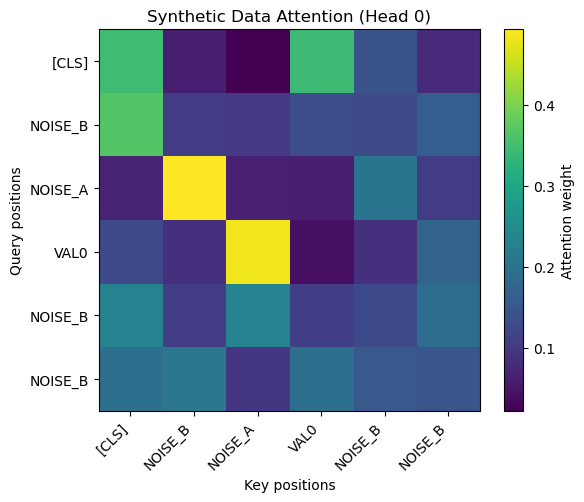
\includegraphics[width=0.5\linewidth]{output.png}
\end{figure}

\end{enumerate}
	\end{enumerate}
\end{solution}


\newpage



\begin{problem}[Autoencoders, 76 pts]
Suppose we want to compress our data into a lower-dimensional representation. What is a principled way to do this with machine learning, such that we can be confident the compression retains as much useful information as possible?

\begin{enumerate}
        \item The Autoencoder. 
        
We can turn this into a game between two networks. An \textit{encoder} $f_\phi : \mathbb R^n \to \mathbb R^d$ takes an input $\mathbf x$ and compresses it down to $d$ dimensions: $\mathbf z = f_\phi(\mathbf x)$. A \textit{decoder} $g_\theta : \mathbb R^d \to \mathbb R^n$ must then reconstruct the original input from just this compressed representation: $\hat{\mathbf x} = g_\theta(\mathbf z)$. We measure how well the decoder succeeds by comparing $\hat{\mathbf x}$ to $\mathbf x$, and backpropagate through both networks:
\[
  \mathcal{L}_{\mathrm{recon}} = \frac{1}{N}\sum_{i=1}^{N} \|\mathbf x_i - g_\theta(f_\phi(\mathbf x_i))\|^2.
\]
This is the \textit{reconstruction loss}, and it is the core of how autoencoders are trained. The logic is simple: if the decoder can faithfully recover $\mathbf x$ from $\mathbf z$, then $\mathbf z$ must have captured the essential structure of $\mathbf x$.

Note that what makes a model an ``autoencoder'' is this encoder--decoder coupling trained with a reconstruction loss---not any particular architecture. The encoder and decoder can be MLPs, CNNs, Transformers, or anything else. It is the training paradigm that defines the autoencoder.

\begin{enumerate}

\item \textbf{Implementation}[12 pts]. In the notebook, implement a convolutional autoencoder on CelebA. Train it, and provide your training and test loss curves. Display the first 5 test images alongside their reconstructions.

\item \textbf{Sampling}[4 pts]. In the notebook, sample random vectors $\mathbf z \sim \mathcal{N}(\bm{0}, \mathbf{I})$ from the autoencoder's latent space and decode them. Do the outputs look like faces? In 1--2 sentences, explain why the autoencoder has no reason to make its latent space produce coherent outputs when sampled this way.
\end{enumerate}
\item The autoencoder gives us a compressed representation, but its latent space has no structure that would let us \textit{generate} new data. What if, instead of learning point embeddings, we tried to learn the probability distribution over images, and then sample from it?

The natural objective is maximum likelihood: given a generative model with latent variables $\bz$ and a prior $p(\bz) = \mathcal{N}(\bm{0}, \mathbf{I})$, the log-likelihood of a datapoint $\bx$ is
\[
  \log p(\bx) = \log \int p(\bx, \bz)\, d\bz = \log \int p(\bx \mid \bz)\, p(\bz)\, d\bz.
\]

To train this model via maximum likelihood, we would need the true posterior $p(\bz \mid \bx)$. By Bayes' theorem,
\[
  p(\bz \mid \bx) = \frac{p(\bx \mid \bz)\, p(\bz)}{p(\bx)}.
\]
However, computing $p(\bx)$ (the evidence) requires evaluating the integral above over all possible values of $\bz$, which is intractable when $p(\bx \mid \bz)$ is parameterized by a neural network in high dimensions.

\begin{enumerate}

\item \textbf{Intractability}[4 pts]. In 1--2 sentences, explain concretely why the integral $\int p(\bx \mid \bz)\,p(\bz)\,d\bz$ is intractable. Why can't we just estimate it by drawing samples $\bz^{(k)} \sim p(\bz)$ and averaging $p(\bx \mid \bz^{(k)})$?
\end{enumerate}

Since we can't compute $p(\bz \mid \bx)$ exactly, we introduce a neural network $q_\phi(\bz \mid \bx)$ that serves as an \textit{approximate posterior}---our best learned guess at the true posterior. To measure how well $q_\phi(\bz \mid \bx)$ approximates $p(\bz \mid \bx)$, we use the Kullback--Leibler (KL) divergence and once again need a clever technique:
\[
  \KL\!\big(q_\phi(\bz \mid \bx) \,\|\, p(\bz \mid \bx)\big) = \E_{q_\phi(\bz \mid \bx)}\!\Big[\log q_\phi(\bz \mid \bx) - \log p(\bz \mid \bx)\Big].
\]

\begin{enumerate}
\setcounter{enumii}{1}
\item \textbf{Deriving the ELBO.} Starting from the KL divergence above:

\begin{enumerate}
  \item \textbf{Expanding} [8 pts]. Expand $\log p(\bz \mid \bx)$ using Bayes' rule, and rearrange to show:
  \[
    \log p(\bx) = \KL\!\big(q_\phi(\bz \mid \bx) \,\|\, p(\bz \mid \bx)\big) + \E_{q_\phi(\bz \mid \bx)}\!\Big[\log p(\bx, \bz) - \log q_\phi(\bz \mid \bx)\Big].
  \]

  \item \textbf{Interpretation} [4 pts]. We define the second term to be the \textbf{Evidence Lower Bound (ELBO)}:
  \[
    \mathrm{ELBO} = \E_{q_\phi(\bz \mid \bx)}\!\Big[\log p(\bx, \bz) - \log q_\phi(\bz \mid \bx)\Big].
  \]
  Since $\KL \geq 0$, conclude that $\mathrm{ELBO} \leq \log p(\bx)$. In one sentence, explain why this means maximizing the ELBO is a sensible surrogate for maximizing the intractable log-likelihood.

  \item\textbf{Rewriting} [8 pts]. Now show that the ELBO can be rewritten as:
  \[
    \mathrm{ELBO} = \E_{q_\phi(\bz \mid \bx)}\!\big[\log p(\bx \mid \bz)\big] - \KL\!\big(q_\phi(\bz \mid \bx) \,\|\, p(\bz)\big).
  \]
  (Hint: split $\log p(\bx, \bz) = \log p(\bx \mid \bz) + \log p(\bz)$.)

\end{enumerate}

\item \textbf{Interpreting the VAE loss.} The loss we minimize is the negative ELBO:
\[
  \mathcal{L}_{\mathrm{VAE}} = -\E_{q_\phi(\bz \mid \bx)}\!\big[\log p(\bx \mid \bz)\big] + \KL\!\big(q_\phi(\bz \mid \bx) \,\|\, p(\bz)\big).
\]

\begin{enumerate}
  \item \textbf{Interpretation}[4 pts]. The first term is the (negative) expected log-likelihood of $\bx$ given samples from the encoder. In 1--2 sentences, explain how this connects back to the reconstruction loss from Section 1. What does minimizing it encourage?

  \item \textbf{Interpretation}[4 pts]. The second term penalizes the encoder's output distribution $q_\phi(\bz \mid \bx)$ for deviating from the prior $p(\bz) = \mathcal{N}(\bm{0}, \mathbf{I})$. Explain how this term addresses the problem you identified in question 1(b): why does it give the model an incentive to organize the latent space for generation?

  \item \textbf{Tensity}[4 pts]. These two terms pull in opposite directions. In 1--2 sentences, describe the qualitative effect of this tension on the VAE's reconstructions and generated samples, compared to the standard autoencoder.
\end{enumerate}

\end{enumerate}
\item VAE Implementation
%% ============================================================

In a VAE, the encoder outputs the parameters of the approximate posterior\\ $q_\phi(\bz \mid \bx) = \mathcal{N}(\bm{\mu}_\phi(\bx),\, \mathrm{diag}(\bm{\sigma}_\phi^2(\bx)))$. That is, a shared convolutional backbone produces a feature vector, which is then projected through two separate linear heads: one outputting $\bm{\mu} \in \R^d$ and one outputting $\log \bm{\sigma}^2 \in \R^d$. During training, we sample $\bz$ from this distribution; during generation, we sample $\bz \sim \mathcal{N}(\bm{0}, \mathbf{I})$ and decode.

\begin{enumerate}

\item \textbf{Reparameterization}[8 pts]. We need to backpropagate through the sampling step $\bz \sim q_\phi(\bz \mid \bx)$, but sampling is not differentiable.
 In 1--2 sentences, explain why we can't directly backpropagate gradients through a sampling operation with respect to the distribution's parameters.
  Show that if $\bm{\epsilon} \sim \mathcal{N}(\bm{0}, \mathbf{I})$, then $\bz = \bm{\mu}_\phi(\bx) + \bm{\sigma}_\phi(\bx) \odot \bm{\epsilon}$ has distribution $q_\phi(\bz \mid \bx)$, and explain briefly why this makes the loss differentiable w.r.t.\ $\phi$.

\item \textbf{Closed-form KL}[6 pts]. Derive the closed-form expression for the KL term when $q = \mathcal{N}(\bm{\mu}, \mathrm{diag}(\bm{\sigma}^2))$ and $p = \mathcal{N}(\bm{0}, \mathbf{I})$:
\[
  \KL(q \| p) = \frac{1}{2}\sum_{j=1}^{d}\Big(\mu_j^2 + \sigma_j^2 - \ln \sigma_j^2 - 1\Big).
\]
(Hint: work coordinate-by-coordinate. Use $\E[z_j] = \mu_j$ and $\E[z_j^2] = \mu_j^2 + \sigma_j^2$.)

\item \textbf{Implementation}[12 pts]. In the notebook, implement a VAE using the architecture described above. Train it, and provide your training and test loss curves (decomposed into reconstruction and KL terms). Display the first 5 test images alongside their reconstructions. Then, sample from $\mathcal{N}(\bm{0}, \mathbf{I})$ and decode---do the samples look like faces? Compare to your results from 1(b).

\end{enumerate}
\end{enumerate}
\end{problem}
\begin{solution}
	\begin{enumerate}
	    \item \begin{enumerate}
	        \item Train VS Test Loss \begin{figure}[H]
	            \centering
	            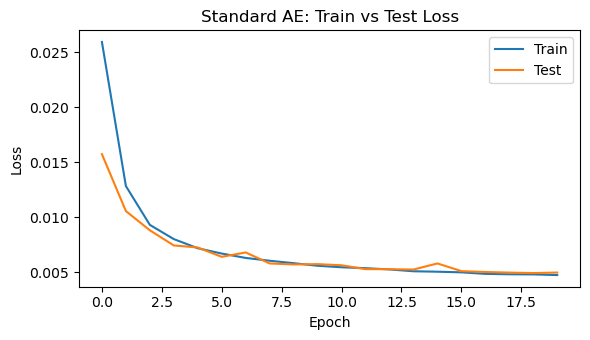
\includegraphics[width=0.5\linewidth]{TrainVSLoss.png}
                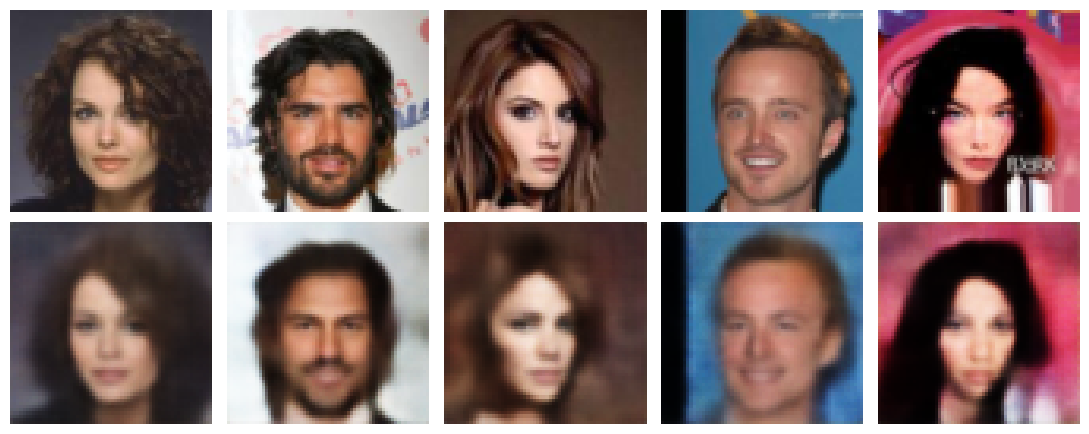
\includegraphics[width=0.5\linewidth]{5images.png}
	        \end{figure}
            \item The autoencoder is trained solely to minimize reconstruction error, so it only needs to ensure that the specific latent codes produced by the encoder map back to valid faces, and has no constraint on what the decoder does with arbitrary points in latent space, additionally, since there is no regularization term, random samples from a standard Gaussian will mostly land outside that region, producing incoherent outputs.
	    \end{enumerate}
        \item \begin{enumerate}
            \item The integral
\[
p(x)=\int p(x\mid z)\,p(z)\,dz
\]
is intractable because it is a high-dimensional integral over all possible latent vectors \(z\), and when \(p(x\mid z)\) is defined by a neural network there is no closed-form expression that lets us evaluate it exactly. In principle we could approximate it with samples \(z^{(k)}\sim p(z)\), but in high dimensions almost all samples from the prior produce values of \(p(x\mid z^{(k)})\) that are  small for a fixed datapoint \(x\), so the estimator has extremely high variance and would require a large number of samples to be accurate.
            \item \begin{enumerate}
                \item Starting from
\[
D_{\mathrm{KL}}\!\left(q_\phi(z\mid x)\,\|\,p(z\mid x)\right)
=
\mathbb{E}_{q_\phi(z\mid x)}
\left[
\log q_\phi(z\mid x)-\log p(z\mid x)
\right],
\]
we expand \(\log p(z\mid x)\) using Bayes' rule:
\[
p(z\mid x)=\frac{p(x,z)}{p(x)},
\qquad\text{so}\qquad
\log p(z\mid x)=\log p(x,z)-\log p(x).
\]

Substituting this gives
\[
D_{\mathrm{KL}}\!\left(q_\phi(z\mid x)\,\|\,p(z\mid x)\right)
=
\mathbb{E}_{q_\phi(z\mid x)}
\left[
\log q_\phi(z\mid x)-\bigl(\log p(x,z)-\log p(x)\bigr)
\right].
\]

Distribute the minus sign:
\[
D_{\mathrm{KL}}\!\left(q_\phi(z\mid x)\,\|\,p(z\mid x)\right)
=
\mathbb{E}_{q_\phi(z\mid x)}
\left[
\log q_\phi(z\mid x)-\log p(x,z)+\log p(x)
\right].
\]

Since \(\log p(x)\) does not depend on \(z\), it can be taken outside the expectation:
\[
D_{\mathrm{KL}}\!\left(q_\phi(z\mid x)\,\|\,p(z\mid x)\right)
=
\mathbb{E}_{q_\phi(z\mid x)}
\left[
\log q_\phi(z\mid x)-\log p(x,z)
\right]
+\log p(x).
\]

Now rearrange:
\[
\log p(x)
=
D_{\mathrm{KL}}\!\left(q_\phi(z\mid x)\,\|\,p(z\mid x)\right)
+
\mathbb{E}_{q_\phi(z\mid x)}
\left[
\log p(x,z)-\log q_\phi(z\mid x)
\right].
\]

Thus,
\[
\boxed{
\log p(x)
=
D_{\mathrm{KL}}\!\left(q_\phi(z\mid x)\,\|\,p(z\mid x)\right)
+
\mathbb{E}_{q_\phi(z\mid x)}
\left[
\log p(x,z)-\log q_\phi(z\mid x)
\right]
}
\]

                \item Since
\[
\log p(x)
=
D_{\mathrm{KL}}\!\left(q_\phi(z\mid x)\,\|\,p(z\mid x)\right)
+
\mathrm{ELBO},
\]
and KL divergence is always nonnegative,
\[
D_{\mathrm{KL}}\!\left(q_\phi(z\mid x)\,\|\,p(z\mid x)\right)\ge 0,
\]
it follows that
\[
\mathrm{ELBO}\le \log p(x).
\]

Thus, the ELBO is a lower bound on the true log-likelihood. Maximizing the ELBO  pushes this lower bound upward toward \(\log p(x)\), tgherefore increasing the data likelihood while also encouraging \(q_\phi(z\mid x)\) to be close to the true posterior \(p(z\mid x)\).
                \item Starting from the definition
\[
\mathrm{ELBO}
=
\mathbb{E}_{q_\phi(z\mid x)}
\left[
\log p(x,z)-\log q_\phi(z\mid x)
\right],
\]
use 
\[
\log p(x,z)=\log p(x\mid z)+\log p(z).
\]
Substituting this in, we get
\[
\mathrm{ELBO}
=
\mathbb{E}_{q_\phi(z\mid x)}
\left[
\log p(x\mid z)+\log p(z)-\log q_\phi(z\mid x)
\right].
\]

 split the expectation
\[
\mathrm{ELBO}
=
\mathbb{E}_{q_\phi(z\mid x)}[\log p(x\mid z)]
+
\mathbb{E}_{q_\phi(z\mid x)}
\left[
\log p(z)-\log q_\phi(z\mid x)
\right].
\]


\[
\mathbb{E}_{q_\phi(z\mid x)}
\left[
\log p(z)-\log q_\phi(z\mid x)
\right]
=
-
\mathbb{E}_{q_\phi(z\mid x)}
\left[
\log q_\phi(z\mid x)-\log p(z)
\right].
\]
By the definition of KL divergence,
\[
D_{\mathrm{KL}}\!\left(q_\phi(z\mid x)\,\|\,p(z)\right)
=
\mathbb{E}_{q_\phi(z\mid x)}
\left[
\log q_\phi(z\mid x)-\log p(z)
\right].
\]
Therefore,
\[
\mathbb{E}_{q_\phi(z\mid x)}
\left[
\log p(z)-\log q_\phi(z\mid x)
\right]
=
-
D_{\mathrm{KL}}\!\left(q_\phi(z\mid x)\,\|\,p(z)\right).
\]

Hence, \[
\boxed{
\mathrm{ELBO}
=
\mathbb{E}_{q_\phi(z\mid x)}[\log p(x\mid z)]
-
D_{\mathrm{KL}}\!\left(q_\phi(z\mid x)\,\|\,p(z)\right)
}.
\]
            \end{enumerate}
            \item \begin{enumerate}
                \item It measures how well the decoder can reconstruct the input \(x\) from a latent sample \(z \sim q_\phi(z\mid x)\). Minimizing it makes the encoder and decoder to preserve the information in \(x\) that is necessary for accurate reconstruction, just like a standard autoencoder tries to make its output match the input.
                \item The KL term prevents the encoder from assigning each input \(x\) to an arbitrary, isolated point in latent space, because it pushes every posterior \(q_\phi(z\mid x)\) to stay close to the shared prior \(p(z)=\mathcal{N}(0,I)\). Hence, the latent codes for different datapoints are forced to take a common, smooth structured region where sampling from the prior makes it appear in areas the decoder has been trained on, which makes generation of new data possible.
                \item  IN the VAE these two terms push the model into the directions described in i) and ii) above. Compared to a standard autoencoder, this yields either less exact reconstructions, but produces a smoother latent space and therefore more coherent samples when generating new data.
            \end{enumerate}
        \end{enumerate}
    \item \begin{enumerate}
        \item Directly sampling \(z \sim q_\phi(z\mid x)\) is not differentiable with respect to \(\phi\) because the random draw introduces stochasticity that can't be represented as a smooth function of \(\mu_\phi(x)\) and \(\sigma_\phi(x)\). Thus, small changes in the parameters do not correspond to an ordinary differentiable path through the sampled value.

We can fix thsi by, let
\[
\epsilon \sim \mathcal{N}(0,I),
\]
and define
\[
z = \mu_\phi(x) + \sigma_\phi(x)\odot \epsilon,
\]
where \(\odot\) denotes elementwise multiplication.

We now show that \(z\) has distribution
\[
q_\phi(z\mid x)=\mathcal{N}\!\left(\mu_\phi(x), \operatorname{diag}(\sigma_\phi^2(x))\right).
\]

Since \(\epsilon \sim \mathcal{N}(0,I)\), each coordinate \(\epsilon_i\) is independent with
\[
\epsilon_i \sim \mathcal{N}(0,1).
\]
Therefore, for each coordinate \(i\),
\[
z_i = \mu_{\phi,i}(x) + \sigma_{\phi,i}(x)\epsilon_i.
\]
A Gaussian is again Gaussian so
\[
z_i \sim \mathcal{N}\!\left(\mu_{\phi,i}(x), \sigma_{\phi,i}^2(x)\right).
\]
Because the coordinates of \(\epsilon\) are independent, the coordinates of \(z\) are also independent, hence
\[
z \sim \mathcal{N}\!\left(\mu_\phi(x), \operatorname{diag}(\sigma_\phi^2(x))\right)
=
q_\phi(z\mid x).
\]

This makes the loss differentiable with respect to \(\phi\) because the randomness is isolated in \(\epsilon\), which is independent of the parameters, while \(z\) is now written as a differentiable function of \(\mu_\phi(x)\) and \(\sigma_\phi(x)\). Therefore gradients can pass through
\[
z = \mu_\phi(x) + \sigma_\phi(x)\odot \epsilon
\]
using  backpropagation.
        \item Let
\[
q(z)=\mathcal{N}\!\left(\mu,\operatorname{diag}(\sigma^2)\right),
\qquad
p(z)=\mathcal{N}(0,I),
\]
where \(z\in\mathbb{R}^d\), \(\mu=(\mu_1,\dots,\mu_d)\), and \(\sigma^2=(\sigma_1^2,\dots,\sigma_d^2)\).

We want to compute
\[
D_{\mathrm{KL}}(q\|p)
=
\mathbb{E}_{q(z)}\left[\log \frac{q(z)}{p(z)}\right].
\]

Because both distributions factor across coordinates,
\[
q(z)=\prod_{j=1}^d q_j(z_j),
\qquad
p(z)=\prod_{j=1}^d p_j(z_j),
\]
with
\[
q_j(z_j)=\mathcal{N}(\mu_j,\sigma_j^2),
\qquad
p_j(z_j)=\mathcal{N}(0,1).
\]
Therefore,
\[
D_{\mathrm{KL}}(q\|p)
=
\sum_{j=1}^d D_{\mathrm{KL}}(q_j\|p_j).
\]

So it suffices to compute the one-dimensional KL divergence. For a single coordinate \(j\),
\[
q_j(z_j)=\frac{1}{\sqrt{2\pi\sigma_j^2}}
\exp\!\left(-\frac{(z_j-\mu_j)^2}{2\sigma_j^2}\right),
\]
and
\[
p_j(z_j)=\frac{1}{\sqrt{2\pi}}
\exp\!\left(-\frac{z_j^2}{2}\right).
\]

Hence,
\[
\log q_j(z_j)
=
-\frac{1}{2}\log(2\pi\sigma_j^2)
-\frac{(z_j-\mu_j)^2}{2\sigma_j^2},
\]
\[
\log p_j(z_j)
=
-\frac{1}{2}\log(2\pi)
-\frac{z_j^2}{2}.
\]

Subtracting,
\[
\log \frac{q_j(z_j)}{p_j(z_j)}
=
-\frac{1}{2}\log \sigma_j^2
-\frac{(z_j-\mu_j)^2}{2\sigma_j^2}
+\frac{z_j^2}{2}.
\]

Now take expectation with respect to \(z_j\sim q_j\):
\[
D_{\mathrm{KL}}(q_j\|p_j)
=
\mathbb{E}_{q_j}\left[
-\frac{1}{2}\log \sigma_j^2
-\frac{(z_j-\mu_j)^2}{2\sigma_j^2}
+\frac{z_j^2}{2}
\right].
\]

Since \(\log \sigma_j^2\) is constant,
\[
D_{\mathrm{KL}}(q_j\|p_j)
=
-\frac{1}{2}\log \sigma_j^2
-\frac{1}{2\sigma_j^2}\mathbb{E}_{q_j}\!\left[(z_j-\mu_j)^2\right]
+\frac{1}{2}\mathbb{E}_{q_j}[z_j^2].
\]

Now use
\[
\mathbb{E}_{q_j}\!\left[(z_j-\mu_j)^2\right]=\sigma_j^2,
\qquad
\mathbb{E}_{q_j}[z_j^2]=\mu_j^2+\sigma_j^2.
\]
Therefore,
\[
D_{\mathrm{KL}}(q_j\|p_j)
=
-\frac{1}{2}\log \sigma_j^2
-\frac{1}{2\sigma_j^2}(\sigma_j^2)
+\frac{1}{2}(\mu_j^2+\sigma_j^2).
\]
Simplifying,
\[
D_{\mathrm{KL}}(q_j\|p_j)
=
\frac{1}{2}\left(\mu_j^2+\sigma_j^2-\log \sigma_j^2-1\right).
\]

Summing over coordinates \(j=1,\dots,d\),
\[
D_{\mathrm{KL}}(q\|p)
=
\sum_{j=1}^d \frac{1}{2}\left(\mu_j^2+\sigma_j^2-\log \sigma_j^2-1\right).
\]

Thus,
\[
\boxed{
D_{\mathrm{KL}}(q\|p)
=
\frac{1}{2}\sum_{j=1}^d
\left(
\mu_j^2+\sigma_j^2-\ln \sigma_j^2-1
\right)
}.
\]
        \item VAE reconstructions will appear noticeably blurrier than the standard AE reconstructions from Part 1(b because the KL regularization prevents the encoder from encoding precise latent codes. It forces the decoder to average over details. The tradeoff is that the VAE's latent space is better for sampling
        
        \begin{figure}
            \centering
            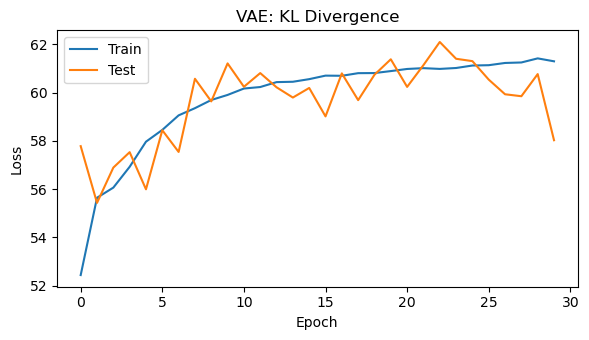
\includegraphics[width=0.5\linewidth]{KL_divergence.png}[H]
            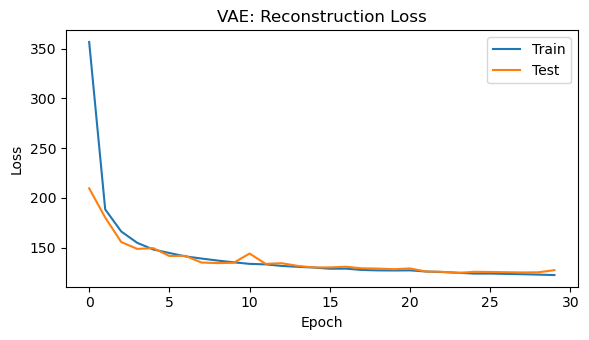
\includegraphics[width=0.5\linewidth]{vae_rec_loss.png}[H]
            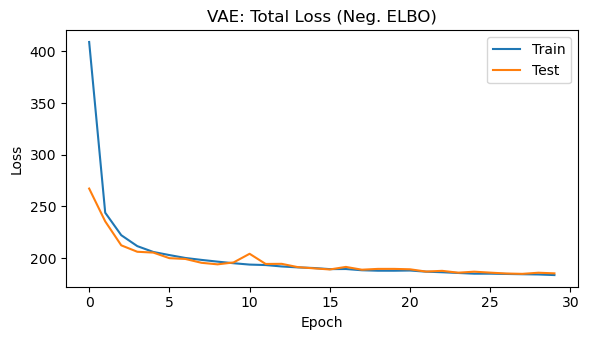
\includegraphics[width=0.5\linewidth]{total_loss.png}[H]
            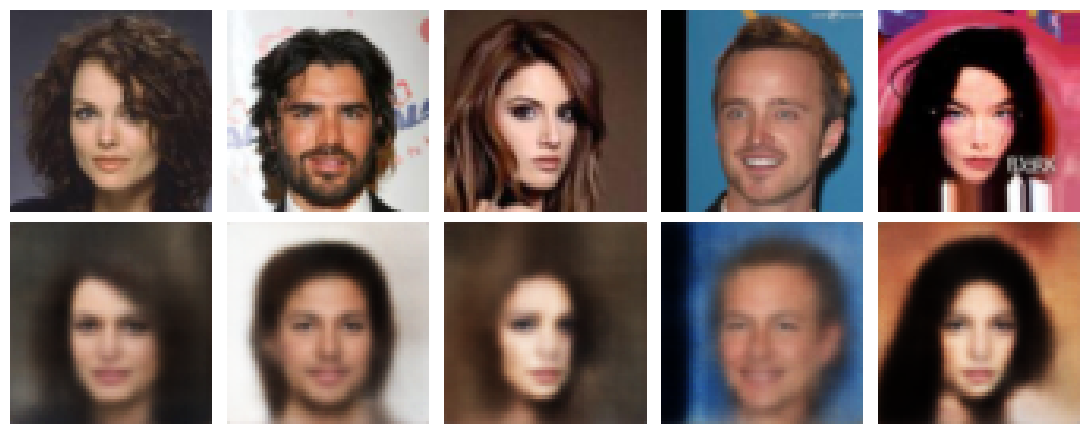
\includegraphics[width=0.5\linewidth]{5imagesvae.png}[H]
        \end{figure}
    \end{enumerate}
	\end{enumerate}
\end{solution}
\newpage

\begin{problem}[Decision Trees, Random Forests and Mixture of Experts]

\noindent
\begin{enumerate}
	\item Suppose we have $B$ independently trained binary classifiers (e.g., decision trees), each with the same accuracy $p > \tfrac{1}{2}$ on a given test point. The ensemble predicts by \textbf{majority vote}.

Let $X$ be the number of trees that predict correctly. Then $X \sim \text{Binomial}(B, p)$, and the ensemble is correct whenever $X > B/2$.

\medskip
\noindent
\textbf{Background: Hoeffding's Inequality.}\quad
Let $Z_1, \ldots, Z_B$ be independent random variables with $Z_i \in [a_i, b_i]$. Hoeffding's inequality states that for the sample mean $\bar{Z} = \frac{1}{B}\sum_{i=1}^{B} Z_i$:
\[
P\!\big(\bar{Z} - \mathbb{E}[\bar{Z}] \leq -t\big) \;\leq\; \exp\!\!\left(\frac{-2B^2 t^2}{\sum_{i=1}^{B}(b_i - a_i)^2}\right).
\]
Intuitively, Hoeffding's inequality is a \emph{concentration inequality}: it says that the average of many bounded independent random variables is unlikely to be far from its expectation, and this probability shrinks \emph{exponentially} in the number of samples $B$. In our setting, each $Z_i \in \{0, 1\}$ indicates whether tree $i$ is correct, so $\bar{Z} = X/B$ and $\mathbb{E}[\bar{Z}] = p$.

\begin{enumerate}
    \item \textbf{[5 points]} Apply Hoeffding's inequality to show that the ensemble error rate satisfies
    \[
    P(X \leq \tfrac{B}{2}) \leq \exp\!\Big({-2B\big(p - \tfrac{1}{2}\big)^2}\Big).
    \]
    \emph{Hint:} The ensemble errs when $\bar{Z} \leq \tfrac{1}{2}$. 

    \item \textbf{[5 points]} Compute the bound for $p = 0.6$ and $B \in \{10, 100, 1000\}$. At what $B$ does the bound first drop below $10^{-6}$? Is that good or necessary?

    \item \textbf{[5 points]} The proof above assumes the trees are \emph{independent}. In practice, bagged trees are trained on overlapping bootstrap samples and are therefore correlated.
    \begin{enumerate}
        \item Explain intuitively why correlation weakens the convergence guarantee.
        \item Random forests add \textbf{feature subsampling} (each split considers only $m$ of $d$ features at random). Explain how this reduces correlation and partially restores convergence.
    \end{enumerate}
\end{enumerate}
\item
Part 1(c) showed that correlation between trees matters. We now make this precise. Suppose we have $B$ trees $T_1, \ldots, T_B$, each with the same prediction variance $\sigma^2 = \text{Var}(T_b(\mathbf{x}))$, and each pair has the same correlation $\rho = \text{Corr}(T_i(\mathbf{x}), T_j(\mathbf{x}))$ for $i \neq j$.

\begin{enumerate}
    \item \textbf{[8 points]} Prove that the variance of the ensemble prediction is:
    \[
    \text{Var}\!\left(\frac{1}{B}\sum_{b=1}^{B} T_b(\mathbf{x})\right) = \rho\,\sigma^2 + \frac{1-\rho}{B}\,\sigma^2.
    \]
    \emph{Hint:} Expand the variance of the sum, separate the diagonal terms ($i = j$) from the off-diagonal terms ($i \neq j$), and use $\text{Cov}(T_i, T_j) = \rho\,\sigma^2$.

    \item \textbf{[4 points]} Analyze the formula:
    \begin{enumerate}
        \item What does the ensemble variance converge to as $B \to \infty$? Can we make the variance arbitrarily small by adding more trees?
        \item What happens when $\rho = 0$? When $\rho = 1$? Relate each case to a practical scenario.
    \end{enumerate}

    \item \textbf{[4 points]} Random forests use $m = \lfloor\sqrt{d}\rfloor$ features per split (for classification). Using the formula from (d), explain why $m = 1$ (one random feature per split) is generally a bad idea, even though it minimizes $\rho$. What tradeoff does $m$ control?
\end{enumerate}

%% ============================================================
\item %% ============================================================
\medskip
\noindent
\textbf{Mixture of Experts (MoE).}\quad
A random forest is a \emph{dense ensemble}: every tree processes every input. A Mixture of Experts is a \emph{sparse ensemble}: a learned gating network routes each input to only a few specialized sub-networks (``experts''), and the output is a weighted combination:
\[
y = \sum_{k=1}^{K} g_k(\mathbf{x})\, E_k(\mathbf{x}), \quad \text{with most } g_k = 0 \text{ (sparse routing)}.
\]
This is the architecture behind many modern LLMs. Sparse MoE allows models to have many more total parameters (and thus more capacity) without proportionally increasing inference cost --- for example, Mixtral 8x7B has ${\sim}47$B total parameters but activates only ${\sim}13$B per token by routing to 2 of 8 experts. Unlike random forest trees, MoE experts \emph{specialize}: the gating network learns to send different types of inputs to different experts.

A key challenge in MoE training is \textbf{expert collapse}, where the gating network funnels most inputs to one or two experts while the rest go unused, wasting capacity. This is typically addressed with an auxiliary \emph{load-balancing loss} that penalizes uneven routing.

\textbf{[4 points]} In 3--5 sentences, compare how random forests and MoE each handle the tradeoff between model capacity and computational cost. Why can a random forest not ``scale up'' in the way that MoE can?
\end{enumerate}

\end{problem}

\begin{solution}
	\begin{enumerate}
	    \item \begin{enumerate}
	        \item Let
\[
Z_i =
\begin{cases}
1 & \text{if tree } i \text{ predicts correctly},\\
0 & \text{otherwise},
\end{cases}
\qquad i=1,\dots,B.
\]
Then the \(Z_i\) are independent, each \(Z_i \in [0,1]\), and
\[
X=\sum_{i=1}^B Z_i,
\qquad
\bar Z = \frac{1}{B}\sum_{i=1}^B Z_i = \frac{X}{B}.
\]
Since each tree has accuracy \(p\),
\[
\mathbb{E}[\bar Z]=p.
\]

The ensemble makes an error when the majority vote is wrong, i.e. when
\[
X \le \frac{B}{2}.
\]
Equivalently,
\[
\bar Z \le \frac{1}{2}.
\]
Thus
\[
\mathbb{P}\!\left(X \le \frac{B}{2}\right)
=
\mathbb{P}\!\left(\bar Z \le \frac{1}{2}\right)
=
\mathbb{P}\!\left(\bar Z - p \le -\left(p-\frac{1}{2}\right)\right).
\]

Now apply Hoeffding’s inequality. Since each \(Z_i \in [0,1]\), we have \(a_i=0\), \(b_i=1\), so
\[
\sum_{i=1}^B (b_i-a_i)^2 = \sum_{i=1}^B 1^2 = B.
\]
Setting
\[
t = p-\frac{1}{2},
\]
Hoeffding gives
\[
\mathbb{P}\!\left(\bar Z - \mathbb{E}[\bar Z] \le -t\right)
\le
\exp\!\left(-\frac{2B^2 t^2}{\sum_{i=1}^B (b_i-a_i)^2}\right)
=
\exp\!\left(-\frac{2B^2 t^2}{B}\right)
=
\exp(-2Bt^2).
\]
Substituting \(t=p-\tfrac12\), we obtain
\[
\mathbb{P}\!\left(X \le \frac{B}{2}\right)
\le
\exp\!\left(-2B\left(p-\frac12\right)^2\right).
\]

Hence,
\[
\boxed{
\mathbb{P}\!\left(X \le \frac{B}{2}\right)
\le
\exp\!\left(-2B\left(p-\frac12\right)^2\right)
}.
\]
            \item Using the bound from part (a),
\[
\mathbb{P}\!\left(X \le \frac{B}{2}\right)
\le
\exp\!\left(-2B\left(p-\frac12\right)^2\right).
\]
For \(p=0.6\),
\[
p-\frac12 = 0.1,
\qquad
\left(p-\frac12\right)^2 = 0.01,
\]
so the bound becomes
\[
\mathbb{P}\!\left(X \le \frac{B}{2}\right)
\le
\exp(-2B\cdot 0.01)
=
\exp(-0.02B).
\]

Now evaluate this for the given values of \(B\):

\[
B=10
\quad\Rightarrow\quad
\exp(-0.02\cdot 10)=\exp(-0.2)\approx 0.8187,
\]

\[
B=100
\quad\Rightarrow\quad
\exp(-0.02\cdot 100)=\exp(-2)\approx 0.1353,
\]

\[
B=1000
\quad\Rightarrow\quad
\exp(-0.02\cdot 1000)=\exp(-20)\approx 2.06\times 10^{-9}.
\]

So the bounds are
\[
\boxed{
\begin{aligned}
B=10 &: \quad \exp(-0.2)\approx 0.8187,\\
B=100 &: \quad \exp(-2)\approx 0.1353,\\
B=1000 &: \quad \exp(-20)\approx 2.06\times 10^{-9}.
\end{aligned}
}
\]

To find when the bound first drops below \(10^{-6}\), solve
\[
\exp(-0.02B)<10^{-6}.
\]
Taking logs,
\[
-0.02B < \ln(10^{-6}) = -6\ln 10.
\]
Thus
\[
B > \frac{6\ln 10}{0.02}.
\]
Using \(\ln 10 \approx 2.3026\),
\[
B > \frac{6(2.3026)}{0.02}\approx 690.78.
\]
Hence the smallest integer \(B\) is
\[
\boxed{B=691.}
\]

This is not especially good as a bound, because Hoeffding’s inequality is a bit loose here and can greatly overestimate the true ensemble error. 
            \item \begin{enumerate}
                \item If the trees are positively correlated, then they tend to make the same mistakes on the same examples so averaging or majority vote does not cancel errors as effectively as in the independent case.  Adding more trees gives less new information, and the ensemble error no longer decreases as quickly with \(B\) as the  Hoeffding bound suggests.
                \item Random forests reduce correlation by forcing different trees, and even different splits within a tree, to consider different random subsets of features rather than always choosing from all \(d\) features. This makes the trees more diverse, so they are less likely to repeatedly make the same split decisions and the same errors, which means majority voting can average out mistakes more effectively and the ensemble regains some of the error reduction that independence would provide.
            \end{enumerate}
	    \end{enumerate}
        \item \begin{enumerate}
            \item Let
\[
\bar T(x)=\frac{1}{B}\sum_{b=1}^B T_b(x).
\]
We want to compute
\[
\operatorname{Var}(\bar T(x)).
\]

Using the variance of a scaled sum,
\[
\operatorname{Var}\!\left(\frac{1}{B}\sum_{b=1}^B T_b(x)\right)
=
\frac{1}{B^2}\operatorname{Var}\!\left(\sum_{b=1}^B T_b(x)\right).
\]
Now expand the variance of the sum:
\[
\operatorname{Var}\!\left(\sum_{b=1}^B T_b(x)\right)
=
\sum_{i=1}^B \operatorname{Var}(T_i(x))
+
\sum_{i\neq j}\operatorname{Cov}(T_i(x),T_j(x)).
\]

By assumption, for every tree,
\[
\operatorname{Var}(T_b(x))=\sigma^2,
\]
so the diagonal terms contribute
\[
\sum_{i=1}^B \operatorname{Var}(T_i(x)) = B\sigma^2.
\]

Also, for \(i\neq j\),
\[
\operatorname{Corr}(T_i(x),T_j(x))=\rho,
\]
and since each tree has variance \(\sigma^2\),
\[
\operatorname{Cov}(T_i(x),T_j(x))
=
\rho \sqrt{\operatorname{Var}(T_i(x))\operatorname{Var}(T_j(x))}
=
\rho \sigma^2.
\]
There are \(B(B-1)\) off-diagonal pairs \((i,j)\) with \(i\neq j\), so
\[
\sum_{i\neq j}\operatorname{Cov}(T_i(x),T_j(x))
=
B(B-1)\rho\sigma^2.
\]

Therefore,
\[
\operatorname{Var}\!\left(\sum_{b=1}^B T_b(x)\right)
=
B\sigma^2 + B(B-1)\rho\sigma^2.
\]
Substitute back:
\[
\operatorname{Var}(\bar T(x))
=
\frac{1}{B^2}\left(B\sigma^2 + B(B-1)\rho\sigma^2\right).
\]


\[
\operatorname{Var}(\bar T(x))
=
\frac{\sigma^2}{B^2}\,B\bigl(1+(B-1)\rho\bigr)
=
\frac{\sigma^2}{B}\bigl(1+(B-1)\rho\bigr).
\]

\[
\operatorname{Var}(\bar T(x))
=
\frac{\sigma^2}{B} + \frac{(B-1)\rho\sigma^2}{B}.
\]

\[
\operatorname{Var}(\bar T(x))
=
\rho\sigma^2 + \frac{1-\rho}{B}\sigma^2.
\]

Hence,
\[
\boxed{
\operatorname{Var}\!\left(\frac{1}{B}\sum_{b=1}^B T_b(x)\right)
=
\rho \sigma^2 + \frac{1-\rho}{B}\sigma^2
}.
\]
            \item \begin{enumerate}
                \item From
\[
\operatorname{Var}\!\left(\frac{1}{B}\sum_{b=1}^B T_b(x)\right)
=
\rho \sigma^2 + \frac{1-\rho}{B}\sigma^2,
\]
take the limit as \(B\to\infty\). Since
\[
\frac{1-\rho}{B}\sigma^2 \to 0,
\]
we get
\[
\lim_{B\to\infty}\operatorname{Var}\!\left(\frac{1}{B}\sum_{b=1}^B T_b(x)\right)
=
\rho\sigma^2.
\]

Thus, the ensemble variance converges to
\[
\boxed{\rho\sigma^2.}
\]
So in general we can't make the variance arbitrarily small just by adding more trees: if \(\rho>0\), there is a nonzero variance floor \(\rho\sigma^2\). Only in the ideal case \(\rho=0\) does the variance go to \(0\) as \(B\to\infty\).
                \item From
\[
\operatorname{Var}\!\left(\frac{1}{B}\sum_{b=1}^B T_b(x)\right)
=
\rho \sigma^2 + \frac{1-\rho}{B}\sigma^2,
\]
consider the two extreme cases.

If \(\rho=0\), then
\[
\operatorname{Var}\!\left(\frac{1}{B}\sum_{b=1}^B T_b(x)\right)
=
\frac{\sigma^2}{B},
\]
which goes to \(0\) as \(B\to\infty\). This corresponds to the case where the trees are uncorrelated, so each tree contributes independent information and averaging greatly reduces variance.

If \(\rho=1\), then
\[
\operatorname{Var}\!\left(\frac{1}{B}\sum_{b=1}^B T_b(x)\right)
=
\sigma^2,
\]
So the ensemble has exactly the same variance as a single tree. This corresponds to the case where all trees are perfectly correlated, meaning they make essentially the same prediction, so adding more trees provides no benefit whatsoever.
            \end{enumerate}
            \item Using fewer features per split tends to reduce the correlation \(\rho\) between trees, which is good for lowering the ensemble variance, but if \(m=1\) then each split is chosen from only a single randomly forced feature, so individual trees become much weaker, and their variance/bias aspects become more bad. Thus \(m\) controls the tradeoff between \emph{tree strength} and \emph{tree correlation}: smaller \(m\) makes trees more diverse but less accurate individually, while larger \(m\) makes trees stronger but also more correlated.
        \end{enumerate}
        \item Random forests scale capacity by adding more trees, but every tree is used for every input, so computation grows linearly with size. On the other hand, MoE models increase capacity with many experts but keep computation low by activating only a small subset per input through sparse routing.
	\end{enumerate}
\end{solution}


\newpage 




\textbf{Name}: Ibrahim Khaliliya

\textbf{Collaborators and Resources}: 
3Blue1Brown Deep Learning chapter 6

\end{document}
